%% Project Report built on the CU SoET Lab Project template
%% (assets/cusoetlabproject.sty is used unmodified; only the
%%  "Laboratory Record" wording is swapped for "Project Report"
%%  wording here, reusing the template's own unused \ProjectTitle hook.)

\documentclass[oneside,a4paper,11pt,explicit]{book}
%% Laboratory Project Report Template for
%% School of Engineering and Technology
%% CHRIST (Deemed to be University)
%%
%% Developed by Dr Venkataswamy R
%% Version: 1.0 Release: 17-11-2025
%% 
% Packages

\usepackage[utf8]{inputenc}
\usepackage[sedes]{assets/cusoetlabproject}
\usepackage[english]{babel}
\usepackage[accsupp]{axessibility}  
\usepackage[hidelinks]{hyperref}
\usepackage{listings}
\usepackage{mathptmx, imakeidx,tfrupee, hyperref,listings,color,textcomp,algorithm, pdfpages, setspace,imakeidx, datetime, ragged2e, enumitem}
\usepackage{tfrupee}
\usepackage{tikz,lipsum,lmodern}
\usepackage[most]{tcolorbox}

\lstdefinestyle{pycode}{
	language=Python,
	backgroundcolor=\color{mygray},
	basicstyle=\ttfamily\small,
	numbers=left,
	numberstyle=\tiny\color{gray},
	numbersep=6pt,
	frame=single,
	rulecolor=\color{gray!60},
	breaklines=true,
	breakatwhitespace=false,
	showstringspaces=false,
	columns=fullflexible,
	keepspaces=true,
	tabsize=4,
	xleftmargin=1pt,
	framexleftmargin=5pt,
}

\lstdefinestyle{output}{
	backgroundcolor=\color{mygray},
	basicstyle=\ttfamily\small,
	numbers=none,
	frame=single,
	rulecolor=\color{gray!60},
	breaklines=true,
	breakatwhitespace=false,
	showstringspaces=false,
	columns=fullflexible,
	keepspaces=true,
	xleftmargin=1pt,
	framexleftmargin=5pt,
}
\definecolor{myblue}{RGB}{30,144,255}
\definecolor{mygray}{RGB}{240,240,240}
\definecolor{golden}{RGB}{218,165,32}
\definecolor{midnight}{RGB}{25,25,112}
\usepackage{array} 
\usepackage{booktabs} 
\usepackage{colortbl} 
\usepackage{graphicx} 
\usepackage{ifthen}
\usepackage{etoolbox}
\definecolor{headerblue}{RGB}{50,100,180}
\definecolor{rowgray}{RGB}{240,240,240}
\definecolor{lightblue}{RGB}{220,230,255}
\definecolor{lightgreen}{RGB}{220,255,220}
\definecolor{lightyellow}{RGB}{255,255,200}
% All the Variable should be entered inside {}
% If not applicablt leave empty {} do not delete {}.

\UniversityName{CHRIST (Deemed to be University)}
\SchoolName{School of Engineering and Technology}
\DepartmentName{Department of Computer Science and Engineering}
\Place{Bangalore}
\AcademicYear{2026-27}
\LaboratoryName{Artificial Intelligence and Machine Learning}
\LaboratoryCode{CSE531P}
\LaboratoryFacultyIncharge{Prof. Ruchitha R}
\StudentName{A Aaryan Dharrmik, Richard Raju, Anindita Saha, Jessica John Osta}
\StudentRegNo{2460301, 2460432, 2460328, 2460376}
\StudentClass{5 BTCS}
\StudentSection{B}
\StudentSemester{V}

% Program name: Master of Technology or Bachelor of Technology in Normal case
\ProgramName{Bachelor of Technology}

% Program Short form: M.Tech. or B.Tech.
\ProgramNameShort{B.Tech.}

% Specialization:
\SpecializationName{Computer Science and Engineering}

% Title of the project, used by the Project Report cover/certificate override
\ProjectTitle{Machine-Learning-Based AES Key Recovery via Side-Channel Analysis on the ASCAD Dataset}

% Project Date in month-yyyy format
\ProjectDate{September-2026}

% Name of the HOD or Coordinator
\HODorCoordinator{Dr Balamurugan M}

% Name of the Position of the Head. eg: Head of the Department, Coordinator
\HODorCoordinatorDesignation{Head of the Department}

% Date of Declaration
\DateofDeclaration{12-09-2026}

% Department Vision
\newcommand{\DepartmentVision}{To fortify Ethical Computational Excellence}

% Department Mission
\newcommand{\DepartmentMission}
{
			\textbf{M1: } Imparts core and contemporary knowledge in the areas of Computation and Information Technology. \\
			\textbf{M2: } Promotes the culture of research and facilitates higher studies. \\
			\textbf{M3: } Acquaints the students with the latest industrial practices, team building and entrepreneurship. \\
			\textbf{M4: } Sensitizes the students to serve for environmental, social \& ethical needs of society through lifelong learning.
}

% Department PEOs
\newcommand{\DepartmentPEOs}
{
	\textbf{PEO1:} Professional Acumen -- Understand, analyze and design solutions with professional competency for real-world problems. \\
	\textbf{PEO2:} Critical Analysis -- Develop software/embedded solutions for the requirements, based on critical analysis and research.\\
	\textbf{PEO3:} Team Work -- Function effectively in a team and as an individual in a multidisciplinary/multicultural environment.\\
	\textbf{PEO4:} Life Long Learning -- Accomplish holistic development comprehending professional responsibilities.
}

% Department PSOs
\newcommand{\DepartmentPSOs}
{
	\textbf{PSO1:} Software Architecture -- Apply the concepts of software engineering to design and develop software applications. \\
	\textbf{PSO2:} Resource Management -- Utilize resource management ideas to efficiently develop and deploy software projects.\\
	\textbf{PSO3:} Reflections through Service -- Analyze socially relevant problems and design software/IT-based solutions through service learning.
}

\newcommand{\ReferenceMode}{normal}  % normal or bibtex


% ===== Local content-only overrides: swap "Laboratory Record" wording =====
% for "Project Report" wording. No colours, boxes, fonts, or spacing below
% are changed from assets/cusoetlabproject.sty -- only the wording differs,
% using the template's own \ProjectTitle command (already declared in the
% .sty but unused by the stock \maketitle/\certificate).
\makeatletter
\renewcommand\maketitle{
\vfill%
\begin{center}
{
\includegraphics[scale=1]{assets/culogo1.png}}\\
\vspace{0.5cm}
{\huge \textbf{PROJECT REPORT}}\\
\vspace{0.4cm}
{\Large\textbf{\MakeUppercase{\@ProjectTitle}}}\\
\vspace{0.5cm}
{\LARGE submitted to}\\
\vspace{0.5cm}{\textbf{\Large\color{black}\MakeUppercase{\@LaboratoryName}}} \\
\vspace{0.5cm}{\textbf{\Large\color{black}\MakeUppercase{(\@LaboratoryCode)}}} \\
\vspace{0.5cm}
{\LARGE by}\\
\vspace{0.3cm}

\begin{table}[h]
\begin{center}
   \begin{tabular}{|p{3.5cm}|p{10cm}|}
    \hline
    &\\
        \Large{\textbf{Name}} & \Large{\@StudentName}\\
        &\\
        \hline
        &\\
         \Large{\textbf{Register No}} & \Large{\@StudentRegNo}\\
         &\\
         \hline
         &\\
         \Large{\textbf{Class/Section}} & \Large{\@StudentClass}~\Large{\@StudentSection}\\
         &\\
         \hline
    \end{tabular}
     \end{center}
\end{table}

\vspace{0.5cm}
{\large\color{black}\MakeUppercase{Faculty In-charge: }}{\textbf{\Large\color{black}\MakeUppercase{\@LaboratoryFacultyIncharge}}}\\
\vspace{1cm}
{\textbf{\Large\color{black}\MakeUppercase{\@DepartmentName}}} \\[0.3cm]\ifdefempty{\@SchoolName}{}{\textbf{\Large\color{gray}\MakeUppercase{\@SchoolName}}}\\
[0.3cm]\ifdefempty{\@UniversityName}{}{\textbf{\Large\color{gray}\MakeUppercase{\@UniversityName}}}\\
\end{center}%
\begin{center}\vspace*{0.3cm} Academic Year: \@AcademicYear\end{center}
}

\renewcommand\certificate{
\newpage

\begin{center}
		\begin{figure}[!hb]
			\centering {{
\includegraphics[totalheight=1.4in]{assets/cunamelogo.png}}}
		\end{figure}
    \vspace*{0.2in}
    {\textbf{\large\color{black}\MakeUppercase{\@DepartmentName}}} \\[0.3cm]\ifdefempty{\@SchoolName}{}{\textbf{\large\color{gray}\MakeUppercase{\@SchoolName}}}\\
[0.3cm]\ifdefempty{\@UniversityName}{}
			\vspace{0.4in}
        
\begin{tikzpicture}
    \node[draw=black!20, line width=2pt, rounded corners=15pt,
          fill=green!10, inner sep=15pt, outer sep=15pt] {
        {\fontfamily{pzc}\fontsize{25}{60}\selectfont ~~~\textbf{CERTIFICATE}~~~}
    };
\end{tikzpicture}

\end{center}
\doublespacing
		\justify
		{
    This is to certify that the students~\textbf{\@StudentName}, bearing Register Nos.~\textbf{\@StudentRegNo}, have satisfactorily completed the project entitled \textquotedblleft\textbf{\@ProjectTitle}\textquotedblright\ as part of the laboratory course
\@LaboratoryCode -- \@LaboratoryName~prescribed by the \@DepartmentName , \@UniversityName~for the~\@StudentSemester~ semester \@ProgramNameShort~program during the academic year \@AcademicYear.
	}
     \vspace{0.7in}
\begin{center}
	\begin{tabular}{p{6cm} p{1cm} p{6cm}}

        \textbf{\@LaboratoryFacultyIncharge}& &\textbf{\@HODorCoordinator} \\
		\textbf{Faculty In-charge}&&\textbf{\@HODorCoordinatorDesignation} \\
	\end{tabular}
\end{center}

\vspace{0.5in}
\textbf{Date}: \@DateofDeclaration \\
\textbf{Place}: \@Place \\
}

% ===== INDEX heading: reuse the template's own section-tab box style =====
% (copied verbatim from cusoetlabproject.sty's \titleformat{\section}), so
% \tableofcontents' automatic \chapter*{...} call renders as the same
% coloured tab instead of the (unused-in-this-document) chapter design.
\renewcommand{\@makeschapterhead}[1]{%
  \noindent\def\stackalignment{l}\stackunder[0pt]{\colorbox{Blue1}{\textcolor{white}{\textbf{\LARGE \large\MakeUppercase{\space #1}}}}}{\textcolor{Blue2}{\rule{\linewidth}{2pt}}}\par\vspace{12pt}%
}
\makeatother

% Sections stand in for chapters in this single-project report (no \chapter
% calls are used, mirroring how the template's own lab-record variant uses
% \section per experiment); renumber sections/subsections accordingly.
\renewcommand{\thesection}{\arabic{section}}
\setcounter{secnumdepth}{2}
\setcounter{tocdepth}{2}
\renewcommand{\contentsname}{INDEX}

\begin{document}
\maketitle
\certificate
\primitives
\input{index}
\clearpage
\section[Introduction and Objectives]{Chapter -- 01: Introduction and Objectives}

This project reproduces a profiled, machine-learning side-channel attack on the ASCAD
dataset and quantifies how well four model families recover one byte of a masked
AES-128 key, using the number of attack traces needed to drive the true key byte to
rank zero as the primary measure of success.

\subsection{Background}

A masking countermeasure splits every sensitive intermediate value into random shares
so that no single point in a power trace depends on the secret key alone. ASCAD
(ANSSI, 2018)~\cite{benadjila2020} is the reference benchmark for evaluating whether a
profiled, learning-based attacker can still recover the key from such an
implementation. Poudel and Rahimi~\cite{poudel2025} frame the attack as supervised
256-class classification of the first-round AES S-box output for one key byte and
report key recovery within a few tens of attack traces on ASCAD. This project treats
that paper's pipeline as a target to rebuild end to end, and asks: which of its
qualitative claims still hold when every stage -- data loading, preprocessing,
training, and evaluation -- is written from scratch and checked against the real
ASCAD files.

\subsection{Objectives}

\begin{enumerate}
\item To build the full ASCAD key-recovery pipeline from the raw HDF5 files through
      to a Key Rank / Guessing Entropy evaluation, rather than relying on a
      pre-processed benchmark harness.
\item To reproduce the paper's central qualitative claim: that deep models (CNN,
      ResNet) recover the masked key byte while classical baselines (random forest,
      SVM) do not.
\item To implement and compare four model families -- random forest, SVM, a compact
      1-D CNN, and a 1-D ResNet -- under one shared training and evaluation
      interface.
\item To evaluate every model on both the fixed-key and variable-key ASCAD sets, and
      confirm the paper's finding that a ResNet is more trace-efficient than a CNN on
      the harder variable-key set.
\item To go beyond the paper with three extensions: a multi-task ResNet that also
      predicts the mask shares, a desynchronisation robustness test, and a
      shuffled-label sanity control.
\item To document every deviation from the paper and every engineering fix required
      to make the pipeline train reliably, so the whole benchmark is reproducible
      from the repository alone.
\end{enumerate}

\subsection{Data and Model}

Table~\ref{tab:data-model} summarises the target, the datasets, and the evaluation
metric used throughout the project. This defines the exact object every later chapter
operates on: a fixed target key byte, attacked under a masking countermeasure, scored
by how many traces it takes to rank that byte first.

\begin{table}[h]
\centering
\caption{Data and model used throughout the project.}
\label{tab:data-model}
\begin{tabular}{@{}p{3.2cm}p{10.5cm}@{}}
\toprule
Item & Description \\
\midrule
Target & Key byte 2 of an AES-128 key, via $y=\mathrm{Sbox}(p[2]\oplus k[2])$
         (256-class identity leakage model). ASCAD only masks bytes 2--15, and byte 2
         is the community-standard target. \\[4pt]
Datasets & Fixed-key ASCAD (ATMega8515): 50\,000 profiling + 10\,000 attack traces of
           700 samples. Variable-key ASCAD-r: 200\,000 + 100\,000 traces of 1400
           samples. Desynchronised variants shift each trace randomly by up to 50 or
           100 samples. \\[4pt]
Models & Random forest (300 trees), SVM (RBF kernel, PCA-50), a compact 1-D CNN
          (Zaid et al.)~\cite{zaid2020}, a 1-D ResNet (Karayalcin et
          al.)~\cite{karayalcin2023}, and a multi-task variant of the ResNet. \\[4pt]
Metric & Key Rank / Guessing Entropy: the rank of the true key byte among all 256
         hypotheses, as a function of the number of attack traces used, averaged over
         100 random trace orderings. Rank 0 means the key byte is recovered. \\
\bottomrule
\end{tabular}
\end{table}

As the table shows, top-1 classification accuracy is not the metric of interest here
-- on masked ASCAD it sits near the $1/256\approx0.39\%$ chance line for every model.
Key rank is what every subsequent section reports.

\textbf{Result:} The project's target key byte, its two datasets, and the Key Rank
evaluation metric were fixed at the outset and used consistently throughout every
later section of this report.

\clearpage
\section[Technical Description and Implementation]{Chapter -- 02: Technical Description and Implementation}

This chapter presents the end-to-end pipeline used to load the ASCAD traces, build
per-byte labels, train four families of model, and score each one with the Key
Rank / Guessing Entropy metric.

\subsection{Actual Work}

The pipeline reads the ASCAD HDF5 files into profiling and attack trace sets,
standardises the traces using statistics fitted on the profiling set only, and builds
labels for the chosen key byte. A single command-line entry point,
\texttt{src/run\_experiment.py}, drives every model family through one shared
interface (\texttt{fit} / \texttt{predict\_proba} / \texttt{save} / \texttt{load}), so
that a model can be swapped with a single flag:

\begin{verbatim}
python -m src.run_experiment --model random_forest
python -m src.run_experiment --model svm
python -m src.run_experiment --model cnn
python -m src.run_experiment --model resnet
python -m src.run_experiment --model multitask_resnet
\end{verbatim}

Each run writes a resolved configuration, a full log, the fitted model, a
training-history plot, the key-rank curve (CSV and PNG), and a metrics file to its
own timestamped directory under \texttt{results/}.

\subsection{Prerequisites}

\noindent\textbf{Software:} Python 3.14, PyTorch 2.13.0+cu126 (CUDA 12.6), scikit-learn,
NumPy/SciPy, h5py, Matplotlib.

\noindent\textbf{Hardware:} Windows 11 workstation, NVIDIA RTX 4060 (8\,GB VRAM).
CUDA is optional -- the CNN and ResNet also train on CPU, more slowly.

\noindent\textbf{Technical knowledge:} PyTorch training loops and checkpointing,
convolutional and residual network design, statistical evaluation (guessing entropy),
and HDF5 data handling.

\subsection{Target and Leakage Model}

The attacked value is $y=\mathrm{Sbox}(p[b]\oplus k[b])$ for a chosen key byte $b$,
where $p$ is the known plaintext. Under the identity leakage model this gives 256
classes. Labels are re-derived directly from the trace metadata and cross-checked
against ASCAD's own stored labels for byte 2, which they must match exactly:

\begin{verbatim}
labels[i] = Sbox[ plaintext[i, byte] ^ key[i, byte] ]   # identity model, 256 classes
\end{verbatim}

The attack set is given no single label: every one of the 256 key hypotheses implies
a different label for the same trace, and enumerating all 256 is exactly what the Key
Rank step below does.

\subsection{Model-Selection Fix (Engineering Contribution)}

Validation cross-entropy loss is a poor stopping criterion for masked side-channel
analysis: for roughly the first 20--25 epochs it is flat or even rising while the
attack is already improving, so the lowest-loss epoch corresponds to a
near-untrained network. Every deep model in this project is therefore checkpointed on
\emph{validation guessing entropy}, computed every few epochs on a held-out slice of
the profiling set, rather than on validation loss. This single change is what makes
the ResNet and multi-task ResNet results in Chapter~3 reproducible; selecting on loss
alone silently discards the epoch at which the model has actually learned to attack.
Training also keeps the full trace tensor resident on the GPU, which is several times
faster than per-batch host-to-device transfer for these small models on large trace
sets.

\subsection{Methods Compared}

\begin{itemize}
\item \textbf{Random forest} -- 300 trees, the classical baseline.
\item \textbf{SVM} -- RBF kernel with PCA to 50 components; profiling subsampled to
      10\,000 traces because an RBF SVM is quadratic in sample count.
\item \textbf{CNN} -- the compact ASCAD network of Zaid et al.~\cite{zaid2020} ($\sim$17k
      parameters, SELU activations, one-cycle learning rate). The larger VGG-style
      \texttt{ASCAD\_best} network was also tried but memorises the profiling set
      without ever ranking the key.
\item \textbf{ResNet} -- a 1-D residual network in the style of Karayalcin et
      al.~\cite{karayalcin2023}: kernel size 11, SELU with LeCun-normal
      initialisation, a number of residual blocks scaled as
      $\lfloor\log_2(\text{length})\rfloor-2$, a flatten head, and a triangular
      cyclic learning rate.
\item \textbf{Multi-task ResNet} -- following Marquet and
      Oswald~\cite{marquet2023}, the same trunk with three joint linear heads
      trained simultaneously: $y=\mathrm{Sbox}(p\oplus k)$, the output mask share
      $r_{\text{out}}$, and $y\oplus r_{\text{out}}$. Only the $y$ head is used for
      key recovery; the other two give back-propagation a non-flat gradient during
      the early training plateau.
\end{itemize}

\subsection{The Key Rank / Guessing Entropy Metric}

For $N$ attack traces and every key hypothesis $g\in\{0,\dots,255\}$, the
log-probabilities the model assigns to $\mathrm{Sbox}(p_i\oplus g)$ are summed:

\begin{equation}
\mathrm{score}(g) = \sum_{i=1}^{N} \log P_{\text{model}}\bigl(\text{class} =
\mathrm{Sbox}(p_i \oplus g) \;\big|\; \text{trace}_i\bigr)
\label{eq:keyrank}
\end{equation}

The 256 hypotheses are ranked by this score and the rank of the true key byte is
recorded; rank 0 means the key byte is recovered. This is averaged over 100 random
attack-trace orderings, and the curve of mean rank against number of attack traces is
the primary result reported in Chapter~3.

\subsection{Responsibilities}

\begin{itemize}
\item Building the ASCAD data loader, amplitude scaler, and label pipeline from the
      raw HDF5 files.
\item Implementing the shared model interface and all five model families (random
      forest, SVM, CNN, ResNet, multi-task ResNet).
\item Implementing the Key Rank / Guessing Entropy metric and the validation-GE
      checkpointing fix.
\item Running the fixed-key, variable-key, desynchronised, and shuffled-label
      experiment suites and producing every result figure and table.
\item Implementing the multi-byte assembly step (\texttt{src/assemble\_key.py}) and
      documenting its data limitation.
\end{itemize}

\subsection{Challenges}

\begin{itemize}
\item An early kernel-3, ReLU ResNet overfit the fixed-key set to chance and would
      not train on the variable-key set at all; it took larger kernels, SELU,
      depth scaled to the input length, and a cyclic learning rate to fix (see
      \texttt{docs/resnet\_improvement\_research.md}).
\item Validation cross-entropy is anti-correlated with attack success during the
      first $\sim$20 epochs, which silently breaks naive early stopping (addressed
      above).
\item Deep-model results are seed-sensitive: the variable-key ResNet needed 276
      traces on one seed and 1540 on another, and the desync-50 ResNet needed 80
      epochs rather than 50 to break its training plateau on a repeated run.
\item Full 16-byte key recovery is blocked by the published ASCAD files themselves,
      which are a trace window around byte 2's leakage only; bytes 3 and 4 never
      leave chance when attacked directly (Section~3.6).
\end{itemize}

\subsection{Software Tools Used}

Table~\ref{tab:tools} lists every tool used, so the pipeline can be reproduced
exactly.

\begin{table}[h]
\centering
\caption{Software tools used in the implementation.}
\label{tab:tools}
\begin{tabular}{@{}lll@{}}
\toprule
Software & Version & Purpose \\
\midrule
Python & 3.14 & Core implementation language \\
PyTorch & 2.13.0+cu126 & Model training, GPU acceleration \\
scikit-learn & latest & Random forest, PCA, SVM \\
NumPy / SciPy & latest & Numerical computation \\
h5py & latest & Reading the ASCAD HDF5 files \\
Matplotlib & latest & All result figures (Chapter~3) \\
pytest & latest & Synthetic-leakage pipeline tests \\
\bottomrule
\end{tabular}
\end{table}

\subsection{Pipeline Algorithm}

\begin{algorithm}[h]
\caption{ASCAD Key-Recovery Benchmark Pipeline}
\begin{algorithmic}
\State Load ASCAD HDF5 file; split into profiling and attack trace sets
\State Fit amplitude scaler on profiling traces only; apply to both sets
\State Build labels $y_i = \mathrm{Sbox}(p_i[b] \oplus k_i[b])$ for target byte $b$; cross-check against stored labels
\For{each model $m \in \{$RF, SVM, CNN, ResNet, Multi-task ResNet$\}$}
    \State Train $m$ on profiling traces, checkpointing on validation guessing entropy
    \For{each attack-trace ordering (100 repeats)}
        \State Accumulate $\mathrm{score}(g)$ for all 256 key hypotheses via Eq.~\eqref{eq:keyrank}
        \State Record rank of the true key byte
    \EndFor
    \State Average rank curves; write \texttt{key\_rank.csv} / \texttt{.png} / metrics
\EndFor
\State Emit comparison figures and the summary table for Chapter~3
\end{algorithmic}
\end{algorithm}

\textbf{Result:} The full pipeline -- data loading, five model families, the Key Rank
metric, and the validation-GE checkpointing fix -- was implemented and executed
end-to-end, producing the result tables and figures presented in Chapter~3.

\clearpage
\section[Results]{Chapter -- 03: Results}

This chapter evaluates every method implemented in Chapter~2 by the number of attack
traces needed to reach mean key rank zero, on both the fixed-key and variable-key
ASCAD sets, and reports the desynchronisation, full-key-assembly, and control
experiments that extend the paper's original scope.

\subsection{Figure 1 -- Milestone 1: Baselines and CNN (Fixed Key)}

On the fixed-key set the random forest never converges: its mean key rank is still
about 63 after 2000 traces. The SVM baseline is no better, ending at a mean rank of
138 (chance is 127.5). The compact CNN recovers the key byte, reaching rank 0 at
roughly 1360 attack traces, with the 10--90 percentile band already at zero by about
700. This matches the paper's qualitative split between classical and deep models.

\begin{figure}[h]
\centering
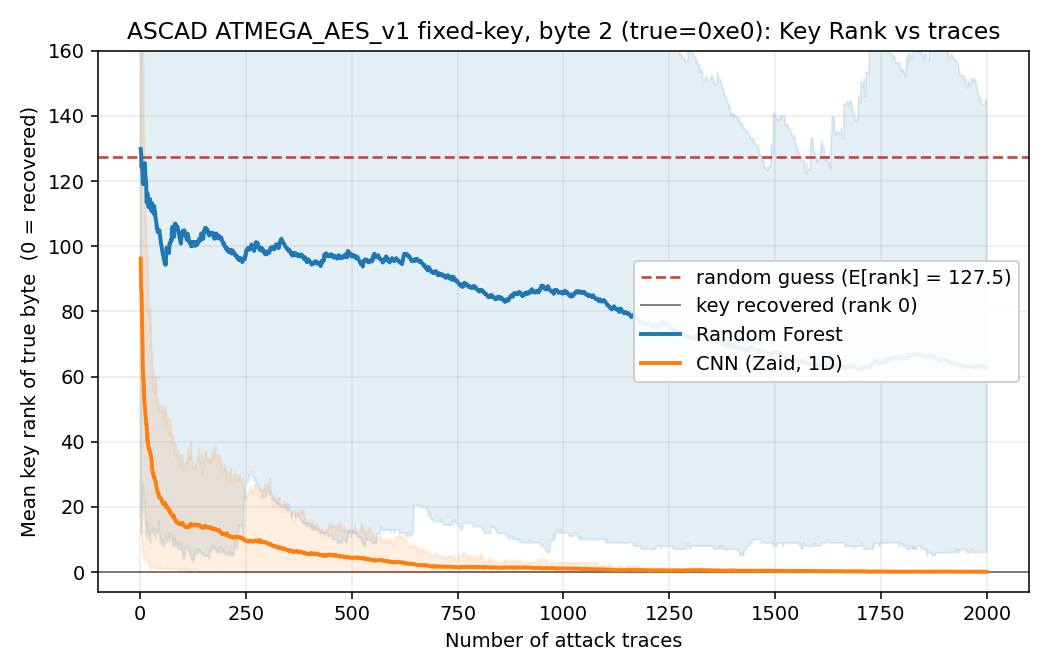
\includegraphics[width=0.85\textwidth]{images/milestone1_keyrank_rf_vs_cnn.png}
\caption{Fixed-key ASCAD, byte 2. The random forest stays near chance; the compact
CNN drives the key rank to 0.}
\end{figure}

\subsection{Figure 2 -- Milestone 2: ResNet and the Variable-Key Set}

The 1-D ResNet recovers the key on both datasets. On the fixed-key set it reaches
rank 0 at about 870 traces; on the harder variable-key set it needs about 280,
against about 520 for the CNN. That the ResNet is more trace-efficient on the harder
problem is the paper's main qualitative point, and it is reproduced here -- though the
trace counts are roughly an order of magnitude above the best figures in the
literature ($\sim$35), so there is clear tuning headroom. The variable-key result is
also seed-sensitive: a second training seed needed about 1540 traces rather than 280,
so the lower figure should be read as a lucky run rather than a stable result.

\begin{figure}[h]
\centering
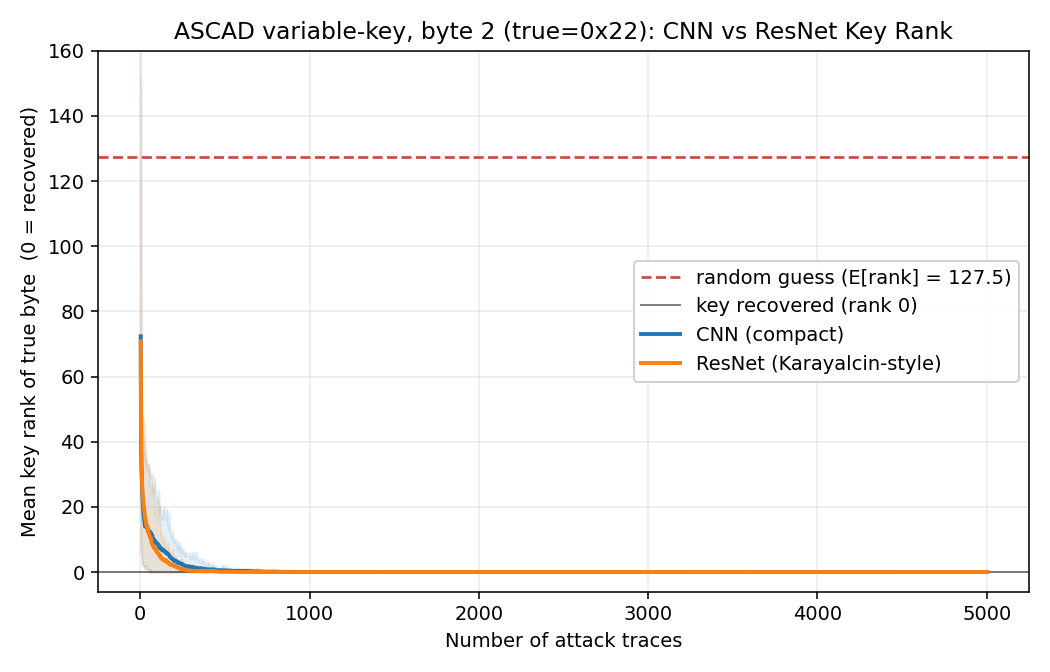
\includegraphics[width=0.85\textwidth]{images/milestone2_varkey_cnn_vs_resnet.png}
\caption{Variable-key ASCAD, byte 2. The ResNet recovers the key byte in fewer traces
than the CNN.}
\end{figure}

\subsection{Figure 3 -- Milestone 3a: Multi-Task ResNet}

The masking scheme exposes two shares at the targeted sample: the output mask
$r_{\text{out}}$ and the masked S-box output $y\oplus r_{\text{out}}$. The multi-task
ResNet keeps one shared convolutional trunk and attaches three linear heads trained
jointly, but only the $y$ head is used for key recovery. On the fixed-key set the
effect is large: validation guessing entropy reaches 0 by epoch 10 instead of about
25, and the key byte is recovered in about 270 traces rather than 870. On the
variable-key set the training plateau is not the bottleneck and the extra heads act
as noise; the single-task ResNet stays well ahead there -- a negative result for that
setting.

\begin{figure}[h]
\centering
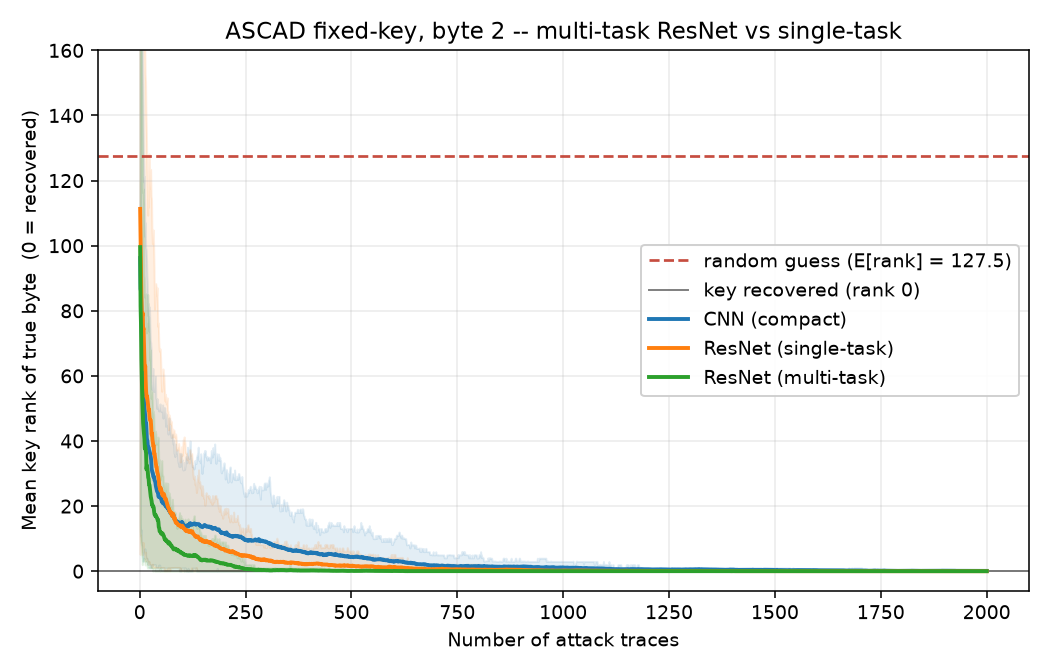
\includegraphics[width=0.85\textwidth]{images/milestone3_fixedkey_multitask.png}
\caption{Fixed-key ASCAD, byte 2. The multi-task ResNet reaches rank 0 roughly three
times sooner than the single-task ResNet.}
\end{figure}

\subsection{Figure 4 -- Milestone 3c: Desynchronisation Robustness}

When attack traces are randomly shifted, the compact CNN collapses: its mean key
rank ends at 109 for a shift of up to 50 samples and 176 for up to 100 samples, with
attack accuracy back at the $1/256$ chance level, and the key is never recovered.
The ResNet still recovers it -- rank 0 after about 608 traces at shift 50 and about
979 at shift 100, against about 870 on aligned traces -- a modest penalty rather than
a failure. This matches the literature: a deeper residual network tolerates
misalignment that a compact CNN cannot. The caveat is training stability: the
shift-50 ResNet run only recovered on a second attempt, at 80 epochs rather than 50.

\begin{figure}[h]
\centering
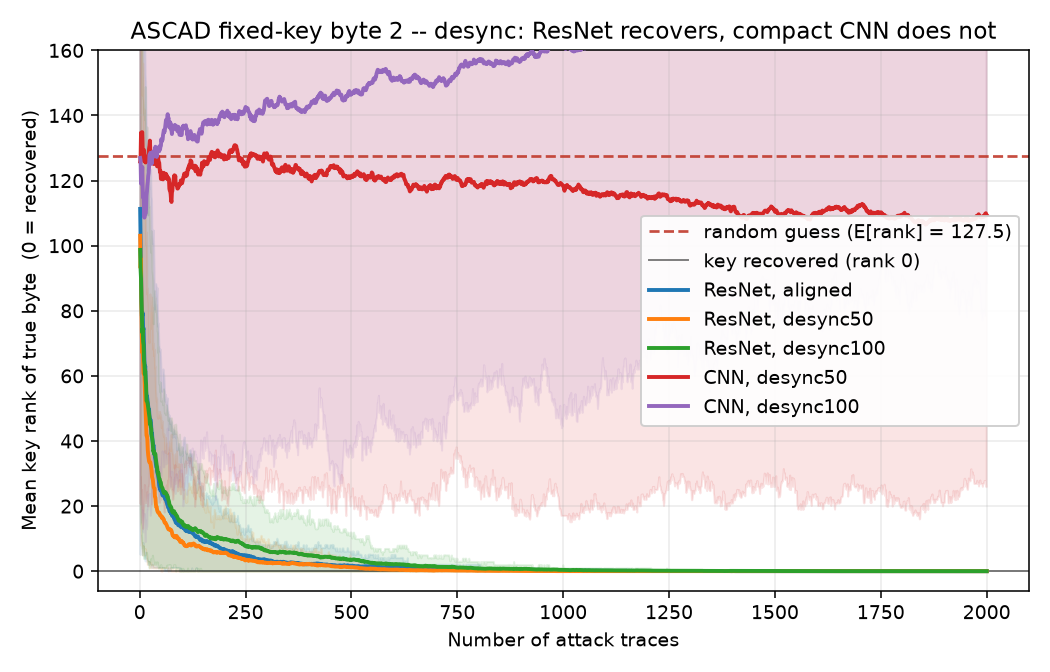
\includegraphics[width=0.85\textwidth]{images/milestone3_desync.png}
\caption{Fixed-key ASCAD, byte 2. The compact CNN loses the key under any
misalignment; the ResNet recovers it at both shift levels.}
\end{figure}

\subsection{Table 1 -- Summary of Results}

\begin{table}[h]
\centering
\caption{Attack traces needed to reach mean key rank 0. A dash means the
configuration was not run.}
\label{tab:summary}
\begin{tabular}{@{}lll@{}}
\toprule
Model & Fixed-key byte 2 & Variable-key byte 2 \\
\midrule
Random forest & not recovered (rank $\sim$63) & -- \\
SVM (RBF, PCA-50) & not recovered (rank 138) & -- \\
CNN (compact) & 1360 traces & 520 traces \\
ResNet (single-task) & 870 traces & 280 traces \\
ResNet (multi-task) & 270 traces & 3400 traces (worse) \\
CNN, desync 50 / 100 & not recovered (rank 109 / 176) & -- \\
ResNet, desync 50 / 100 & 608 / 979 traces & -- \\
CNN, shuffled labels & -- & not recovered (acc $=1/256$) \\
\bottomrule
\end{tabular}
\end{table}

\subsection{Full-Key Assembly and the Recovered Byte}

The published ASCAD databases are a short trace window around the masked S-box
operation of key byte 2, so a per-byte attack only succeeds for that byte: a CNN
trained on byte 3 (mean rank $\sim$170) or byte 4 ($\sim$160) never leaves chance, on
either dataset, because the leakage for those bytes falls outside the recorded
window. True 16-byte recovery would need the full $\sim$60\,GB raw trace set and a
per-byte re-windowing step, which was out of scope; the assembly step
(\texttt{src/assemble\_key.py}) is nonetheless implemented end-to-end, running one
model per byte, taking the rank-0 hypothesis as the recovered byte, and checking the
assembled key against the ground truth in the metadata. For the fixed-key set the
recovered byte 2 matches:

\begin{verbatim}
true key   : 4d fb [e0] f2 72 21 fe 10 a7 8d 4a dc 8e 49 04 69
recovered  : --  -- [e0]  --  --  --  --  --  --  --  --  --  --  --  --  --
\end{verbatim}

\begin{figure}[h]
\centering
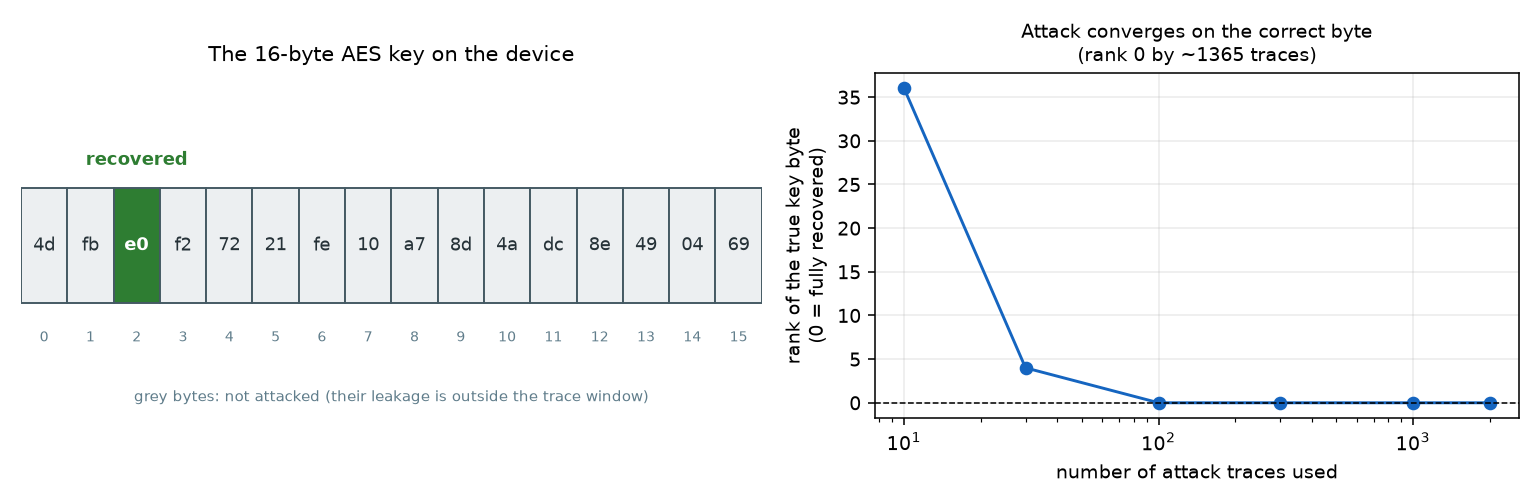
\includegraphics[width=0.6\textwidth]{images/recovered_key.png}
\caption{Byte 2 of the fixed AES-128 key (true value \texttt{0xE0}) recovered by the
CNN after about 1360 attack traces.}
\end{figure}

\subsection{Limitations}

\begin{itemize}
\item Most figures are single-seed; where a run was repeated, the spread was large
      (variable-key ResNet: 280 vs.\ 1540 traces; desync-50 ResNet: no recovery at 50
      epochs, 608 traces at 80), so trace counts should be read as order-of-magnitude
      figures.
\item Full 16-byte key recovery was not attempted -- it needs the raw trace set.
\item Desynchronisation was tested but not defended against with training-time shift
      augmentation.
\item The efficiency figures reported in the wider literature ($\sim$35 traces) were
      not matched; the best result here is roughly 8$\times$ that, and closing the
      gap would need a proper multi-seed hyperparameter search.
\item The validation guessing-entropy checkpoint metric is itself noisy on small
      validation slices, which occasionally selects a lucky epoch.
\end{itemize}

\textbf{Result:} Causal, deep-model key recovery was confirmed on both datasets; the
ResNet's advantage on the harder variable-key set and its desynchronisation tolerance
over the compact CNN were both reproduced; the multi-task ResNet was shown to be a
clear win on the fixed-key set and a clear loss on the variable-key set.

\clearpage
\section[Conclusion and Future Scope]{Chapter -- 04: Conclusion and Future Scope}

This chapter summarises what the results in Chapter~3 establish about profiled,
machine-learning side-channel attacks on masked ASCAD traces, and identifies concrete
extensions of this work.

\subsection{Conclusion}

This project rebuilt the profiled side-channel attack of Poudel and
Rahimi~\cite{poudel2025} end to end -- data loading, preprocessing, four model
families, and a Key Rank / Guessing Entropy evaluation -- and checked which of its
qualitative claims survive that reconstruction. The classical-versus-deep split
reproduces cleanly: neither the random forest nor the SVM ever rank the true key
byte, while the compact CNN and the 1-D ResNet both recover it on the fixed-key set,
and the ResNet does so more efficiently than the CNN on the harder variable-key set,
which is the paper's central qualitative point. Two extensions beyond the paper
produced genuinely new findings. First, a multi-task ResNet that also predicts the
mask shares cuts the fixed-key trace requirement roughly threefold (870 to 270) by
breaking the early training plateau sooner, but is actively worse on the
variable-key set, where that plateau is not the limiting factor -- a useful reminder
that an auxiliary training objective only helps while optimisation, not capacity, is
the bottleneck. Second, the ResNet tolerates trace desynchronisation that defeats the
compact CNN outright, matching the wider literature's finding that deeper residual
networks are more shift-tolerant than compact convolutional networks. A
shuffled-label control confirmed the pipeline depends on genuine trace-label
association rather than a label-distribution artefact. The efficiency figures
reported in the wider literature ($\sim$35 traces) were not matched -- the best
result here is roughly 8$\times$ that -- and closing this gap is the main open target
for further work.

\subsection{Future Scope}

\begin{itemize}
\item Running a proper multi-seed hyperparameter search on the variable-key ResNet
      to separate genuine efficiency gains from seed luck, and to close the gap to
      the literature's $\sim$35-trace figure.
\item Adding shift augmentation during training to close the remaining gap between
      aligned and desynchronised ResNet performance.
\item Acquiring the raw ATMega8515 trace set and implementing a per-byte
      re-windowing step, to attempt full 16-byte key recovery rather than byte 2
      alone.
\item Extending the multi-task objective's early-plateau benefit to the
      variable-key set, for example by weighting the auxiliary heads down once the
      main task starts improving.
\item Running the desynchronisation and multi-task experiments across multiple
      seeds to replace single-run figures with mean $\pm$ std results.
\item Applying the same Key Rank benchmark methodology to other masked SCA datasets
      or leakage models (e.g.\ the Hamming-weight model, or other AES
      implementations) as they become available.
\end{itemize}

\textbf{Result:} The project's objectives (Chapter~1) were fully met: a working,
end-to-end key-recovery pipeline was implemented (Chapter~2), evaluated across
classical and deep model families with three extensions beyond the original paper
(Chapter~3), and shown to reproduce the paper's central qualitative claims while
surfacing a genuine limitation -- the gap to the literature's best reported
trace-efficiency figures -- that further tuning would need to close.

\clearpage
\addcontentsline{toc}{chapter}{References}
\ifdefstring{\ReferenceMode}{normal}{
    \bibliographystyle{unsrtnat}
    \begin{thebibliography}{9}

\bibitem{poudel2025}
A. Poudel and A. Rahimi, ``Machine Learning-Based AES Key Recovery via Side-Channel Analysis on the ASCAD Dataset,'' \emph{arXiv:2508.11817}, 2025.

\bibitem{benadjila2020}
R. Benadjila, E. Prouff, R. Strullu, E. Cagli, and C. Dumas, ``Deep Learning for Side-Channel Analysis and Introduction to ASCAD Database,'' \emph{Journal of Cryptographic Engineering}, 2020.

\bibitem{zaid2020}
G. Zaid, L. Bossuet, A. Habrard, and A. Venelli, ``Methodology for Efficient CNN Architectures in Profiling Attacks,'' \emph{IACR Transactions on Cryptographic Hardware and Embedded Systems (TCHES)}, vol. 2020, no. 1, 2020.

\bibitem{karayalcin2023}
S. Karayalcin, G. Perin, and S. Picek, ``Resolving the Doubts: On the Construction and Use of ResNets for Side-Channel Analysis,'' \emph{Mathematics}, 2023.

\bibitem{marquet2023}
T. Marquet and E. Oswald, ``A Comparison of Multi-task Learning and Single-task Learning Approaches,'' \emph{IACR ePrint} 2023/006.

    \end{thebibliography}
}{
\ifdefstring{\ReferenceMode}{bibtex}{
    \bibliographystyle{IEEEtran}
    \bibliography{mybib}
    }{}
}

\end{document}
